%% Le lingue utilizzate, che verranno passate come opzioni al pacchetto babel. Come sempre, l'ultima indicata sar� quella primaria.
%% Se si utilizzano una o pi� lingue diverse da "italian" o "english", leggere le istruzioni in fondo.
\def\thudbabelopt{italian}
%% Valori ammessi per target: bach (tesi triennale), mst (tesi magistrale), phd (tesi di dottorato).
\documentclass[target=bach]{thud}


\course{Internet of Things, Big Data e Web}
\title{Monitoraggio della batteria di dispositivi Android con IoT}
\author{Alberto Morini}
\supervisor{Prof.\ Ivan Scagnetto}
\date{2021/2022}

%% Campi obbligatori: \title, \author e \course.
%% Altri campi disponibili: \reviewer, \tutor, \chair, \date (anno accademico, calcolato in automatico), \rights
%% Con \supervisor, \cosupervisor, \reviewer e \tutor si possono indicare pi� nomi separati da \and.
%% Per le sole tesi di dottorato:

\contacts{Via San Fermo, 8\\31029 Vittorio Veneto --- Italia\\+39 3456945815\\\texttt{https://github.com/albertomorini}\\\texttt{99morini@gmail.com}}

%% --- Pacchetti consigliati ---
%% pdfx: per generare il PDF/A per l'archiviazione. Necessario solo per la versione finale
\usepackage[a-1b]{pdfx}
%% hyperref: Regola le impostazioni della creazione del PDF... pi� tante altre cose. Ricordarsi di usare l'opzione pdfa.
\usepackage[pdfa]{hyperref}
%% tocbibind: Inserisce nell'indice anche la lista delle figure, la bibliografia, ecc.

%% --- Stili di pagina disponibili (comando \pagestyle) ---
%% sfbig (predefinito): Apertura delle parti e dei capitoli col numero grande; titoli delle parti e dei capitoli e intestazioni di pagina in sans serif.
%% big: Come "sfbig", solo serif.
%% plain: Apertura delle parti e dei capitoli tradizionali di LaTeX; intestazioni di pagina come "big".


\usepackage{listings}
\usepackage{color}

\definecolor{dkgreen}{rgb}{0,0.6,0}
\definecolor{gray}{rgb}{0.5,0.5,0.5}
\definecolor{mauve}{rgb}{0.58,0,0.82}

\lstset{frame=tb,
  language=SQL, %Si, va bene anche per il Java, lasciate SQL credetemi
  aboveskip=3mm,
  belowskip=3mm,
  showstringspaces=false,
  columns=flexible,
  basicstyle={\small\ttfamily},
  numbers=none,
  numberstyle=\tiny\color{gray},
  keywordstyle=\color{blue},
  commentstyle=\color{dkgreen},
  stringstyle=\color{mauve},
  breaklines=true,
  breakatwhitespace=true,
  tabsize=3
}

\begin{document}
\maketitle

%% Dedica (opzionale)
\begin{dedication}
	The sun is shinin', I can look at the horizon\\
	The walls keep gettin' wider, I just hope I never find 'em.\\
	-Wings, Mac Miller.
\end{dedication}


%% Sommario (opzionale)
\abstract

    Nell'ultimo decennio la diffusione di smartphone e tablet si è estesa in tutto il mondo, andando a influenzare la vita privata e lavorativa dell'uomo.\

    Il punto di forza di tali dispositivi risiede nella loro portabilità agevolata dall'alimentazione mediante una batteria ricaricabile, in questo progetto viene trattata la realizzazione di una piattaforma in grado di rilevare il livello di capacità di quest'ultima, quindi mostrarne una panoramica all'utente.

    L'idea è nata dalla necessità di un ristorante che utilizza dei tablet come menù, dove al termine di ogni servizio un cameriere deve controllare lo stato di carica di tutti i dispositivi.\\
    Questa soluzione non si applica solamente alla ristorazione, bensì può trovare spazio in più settori, dall'industria 4.0 a uffici di vario tipo, fino ad arrivare all'uso personale.

    L'Internet delle cose (IoT) è parte integrante del progetto, poiché l'obiettivo è quello di monitorare più apparecchi possibili, sfruttando sensori e componenti già presenti nei device.


%% Indice
\tableofcontents

%% Lista delle tabelle (se presenti)
%\listoftables

%% Lista delle figure (se presenti)
\listoffigures

%% Corpo principale del documento
\mainmatter

%% Parte
%% La suddivisione in parti � opzionale; solitamente sono sufficienti i capitoli.
%\part{Parte}
%%\cite{Knu86} -> thud.bib


%% Capitolo
\chapter{Archittettura concettuale}
    Il progetto, con il nome d'arte 'Byce', si suddivide in due sviluppi: l'applicativo mobile e la piattaforma server, che in quest'ordine rappresentano i componenti del paradigma client-server.

\section{Analisi dei requisiti}
    I requisiti fondamentali al funzionamento del sistema sono i seguenti:

    \begin{enumerate}
        \item Ogni client deve poter rilevare il livello di carica della propria batteria, in seguito, comunicarlo al server tramite messaggi ben definiti.\\
        I dispositivi mobili devono possedere la capacità di autenticare i messaggi inviati mediante l'uso di opportuni meccanismi, infine, è richiesto che ogni smartphone o tablet sia univocamente identificabile.

        \item Il server deve garantire la ricezione simultanea di informazioni provenienti da diversi device, validare l'attendibilità dei messaggi ricevuti e in caso positivo, inserire le informazioni all'interno di un database.\
        La piattaforma deve consentire all'utente di visualizzare i dari rilevati, utilizzando un'infografica che rappresenti chiaramente e senza ambiguità il dato trattato.

        \item \`E necessario che i client possano instaurare una connessione con il server a prescindere della locazione in cui si trovino, quindi è richiesta una tecnologia in grado di sostenere una comunicazione costituita da un canale affidabile e immateriale.
    \end{enumerate}


\section{Casi d'uso}

    L'interazione prevista dall'utente consiste principalmente nell'avvio dei software a lato server e client, in quest'ultimo, durante il primo avvio, sarà fondamentale fornire il consenso ai rispettivi permessi di sistema che verranno richiesti. Se tali permission vengono rifiutate, l'app sarà limitata nelle sue operazioni.\

    Inoltre, alla prima esecuzione del server, l'utente dovrà creare una password la quale verrà memorizzata nel rispettivo file system. Tale password dovrà essere fornita anche ai dispositivi mobili con il compito di rendere attendibili i messaggi che verranno spediti; in assenza di questo input o nel caso fosse errato, l'applicativo non inverà mai i dati, bensì si limiterà a stamparli a video.\

    Infine, l'utente può consultare le informazioni rilevate mediante un sito web, il quale ne offrirà un'opportuna rappresentazione grafica.

    Il sistema è pensato per essere autonomo, quindi a prescindere dall'utilizzo dei device gli applicativi continueranno la loro esecuzione in maniera automatizzata, senza richiedere l'intervento umano.


\graphicspath{ {./img/} }
\begin{figure}[h]
\centering
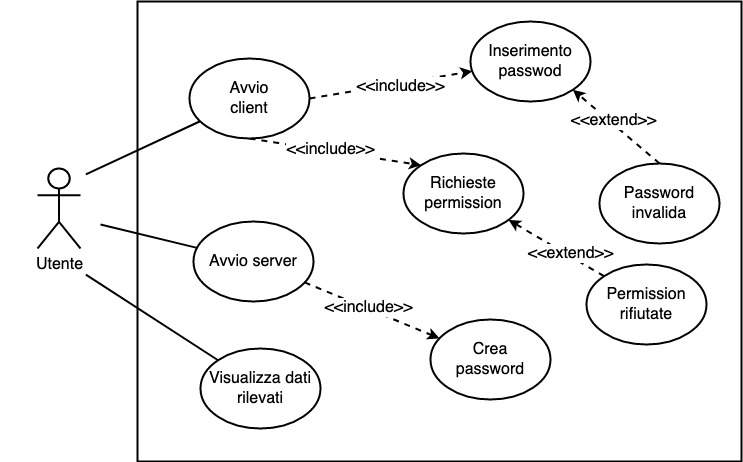
\includegraphics[width=15cm]{useCase}
\caption{Use Case}
\label{fig:usecase}
\end{figure}


\section{Schema delle classi (UML)}

    Le funzioni rese disponibili dai software, sono rappresentate dalle omonime classi nel seguente modello.

    Il server si suddivide in due sotto moduli, il primo adibito all'autenticazione e registrazione dei device, mentre l'altro all'elaborazione dei dati rilevati. Ogni messaggio ricevuto dovrà essere validato per garantire l'attendibilità del mittente.
    L’avvio da parte dell’utente mostrato nel caso d’uso precedente è una singola azione che istanzierà entrambi i processi.


    I dispositivi mobili si occupano di contattare il server opportuno in base all'azione che vogliono compiere. Inoltre ogni device deve ricavare le informazioni relative alla propria batteria, alcuni metadati per collocare l'informazione in uno spazio temporale e i dettagli necessari per poter essere univocamente identificabile, quindi riconoscibile all'utente.
\newpage
    \begin{figure}[h]
    	\centering
    	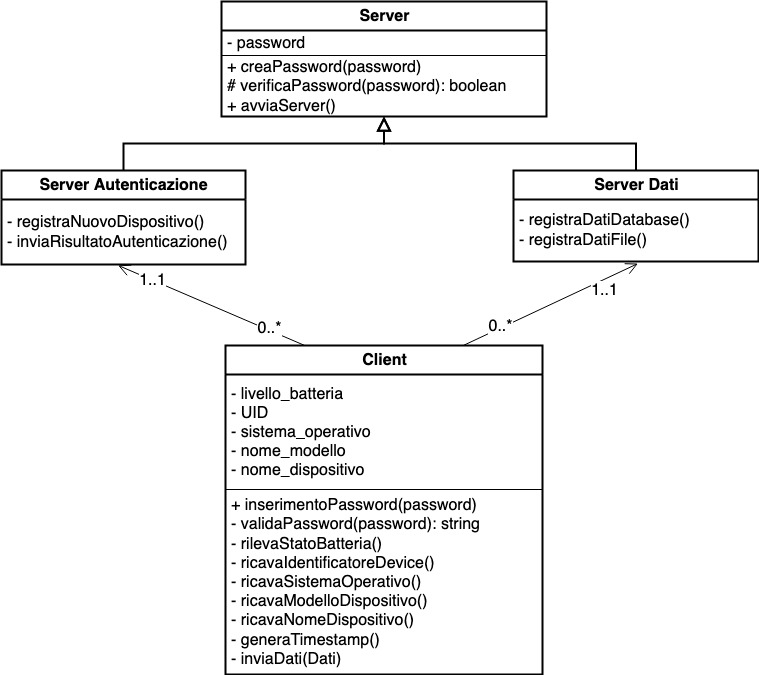
\includegraphics[width=15cm]{uml}
    	\caption{Schema delle classi}
    	\label{fig:uml}
    \end{figure}
    \textit{La visibilità dei metodi e attributi è mostrata verso l'utente.}


\section{Modello di sviluppo}

    La metodologia di sviluppo agile è il cuore della realizzazione di questo progetto, tramite l'approccio incrementale si compone il sistema completo, mentre attraverso le iterazioni delle fasi di analisi, implementazione e validazione, si arricchisce il software in questione di nuove funzionalità.

    Il punto di partenza è la realizzazione dell'applicativo mobile, poiché rappresenta il componente più complesso e critico da costruire. Inizialmente avviene una fase di ricerca delle potenziali tecnologie (quali linguaggi di programmazione, librerie, ecc.) che possano soddisfare i requisiti inviduati, per poi validare le soluzioni mediante opportuni test di prototipazione throw-away\footnote[1]{Prototipazione throw-away: si realizza velocemente un prototipo grezzo e non destinato a diventare la versione finale del prodotto, con il fine di individuare la tecnologia adatta.}.\\
    Poiché il software deve integrarsi e interagire con il server, la realizzazione di quest'ultimo avviene in parallelo adottando le medesime fasi di sviluppo.


\chapter{Stato dell'arte}

    Attualmente nel mercato sono presenti soluzioni simili a quella realizzata, le quali però spesso forniscono funzioni limitate senza offrire un sistema completo.

    \section{IFTTT}

    IFTTT è un'app di proprietà della omonima società, disponibile sia per il sistema operativo Android che per iOS.
    Il software consente all'utente di creare svariate automazioni, compresa la monitorazione del livello della batteria.\\
    Le funzioni offerte variano a seconda dell'abbonamento a cui l'utente è iscritto.

    \begin{enumerate}
        \item La versione gratuita dell'applicativo offre lo sviluppo di massimo 5 automazioni, dove ognuna può essere costituita da al più da 3 operazioni, le quali non consentono personalizzazioni.\\
        Nello specifico, il monitoraggio della batteria è limitato a determinate azioni: il livello di batteria scende al di sotto del 15\%, il dispositivo viene collegato alla corrente o viceversa, scollegato.
        Per ottenere tutte le casistiche citate è necessario quindi creare 3 automazioni distinte, in seguito, è possibile comunicare l'evento monitorato attraverso applicazioni predefinite come ad esempio l'invio di una email, oppure un messaggio di testo.
        \item Le offerte a pagamento, possono entrambe soddisfare i requisiti individuati.
        La differenza principale rispetto al punto precedentemente è l'assenza di limiti nel numero di funzioni, questo comporta maggior facilità nella creazione dei flussi di automazione, inoltre la versione più costosa consente anche la modifica delle funzioni citate poc'anzi.
    \end{enumerate}

    \subsection{Problematiche}

    \`E richiesto che la rete alla quale i device sono connessi abbia un'accesso a Internet, poiché le informazioni inviate vengono processate tramite i server dell'azienda proprietaria.\\
    Questa caratteristica oltre a rappresentare un'ulteriore spesa per l'utente, può comportare una incopatibilità con l'ambiente di installazione, in quanto la connessione a Internet non sempre è disponibile, ci basti pensare a un ristorante in montagna oppure un paese con leggi che ne limitino l'uso.

    Inoltre, l'attraversamento dei dati nei server close source\footnote[1]{Codice close soure: il codice non è disponibile pubblicamente e quindi non analizzabile.} aziendali, può rappresentare una perdita della privacy per l'utente.


    \section{Automate}

    Automate è un'app disponibile unicamente per Android, sviluppata dalla compagnia LlamaLab.

    La versione gratuita offre 30 funzioni chiamati "blocchi" per ogni automazione, mentre l'edizione a pagamento abbatte questo limite, la quale però non è necessaria per raggiungere l'obiettivo prefissato in questa tesi.

    L'applicativo, come il precedente, consente la creazione di flussi di automazione attraverso un'interfaccia grafica inizialmente un po' confusionaria. Il software consente di rilevare lo stato della batteria e inserirlo all'interno di un pacchetto HTTPS\footnote[2]{HTTPS: HyperText Transport Protocol Secure, arricchisce il protocollo HTTP con la crittografia TLS/SSL.} specificando il server che si desidera, quindi anche uno personale.
    Il corpo del messaggio è costituito dal metalinguaggio JSON\footnote[3]{JSON: JavaScript Object Notation standard costituito da dati in coppie attributo-valore, vettori e ulteriori oggetti.}, per identificare il dispositivo è possibile ricavare il MAC address\footnote[4]{MAC address: un codice esadecimale di 48 bit assegnato univocamente dal produttore della scheda di rete.} mediante delle istruzioni a riga di comando\footnote[5]{Istruzioni a riga di comando: un'insieme di parole chiave utilizzate per interagire testualmente con il sistema operativo.}. \\
    Tali azioni possono risultare molto complesse se non impossibili, da eseguire per l'utente comune.


    \section{Apple Shortcuts}

    Nel 2017 Apple acquistò "Shorcuts", un applicativo a pagamento già presente nel proprio store.
    Negli anni il software è stato esteso tramite l'integrazione dell'assistente vocale e ulteriori funzioni.

    Come le soluzioni precedenti, pure Shortcuts consente la creazione di svariate automazioni e quindi, di ricavare lo stato di carica dei soli device prodotti dall'azienda di Cupertino.

    L'idea implementata con questo software è la stessa delle precedenti: si ricava il livello di batteria, lo si comunica mediante applicazioni installate come ad esempio un client di posta oppure tramite la scrittura di un file condiviso su un server.

    \section{Il mercato e Byce}

    Riassumendo, le alternative individuate consentono una maggior flessibilità e personalizzazione rispetto al software creato, tuttavia le soluzioni presentano alcune problematiche comuni, tra cui:

    \begin{enumerate}
        \item Il codice sorgente delle applicazioni non è pubblico, questa scelta pesa negativamente sulla privacy utente, poiché non è possibile validare il corretto comportamento dei programmi.
        \item Lo sviluppo delle automazioni consiste principalmente nell'ideazione di flussi logici, ponendo in cascata varie funzioni esistenti, questa progettazione può rivelarsi complessa per una figura con una debole conoscenza tecnica.
        \item L'assenza di un sistema completo, gli applicativi si limitano a rilevare e inviare l'informazione, senza fornire una soluzione a lato server. La creazione di una piattaforma ad hoc per integrarsi con i software citati può risultare molto complessa a causa della scarsa personalizzazione dei messaggi inviati dai client.
    \end{enumerate}


    \graphicspath{ {./img/} }
    \begin{figure}[h]
        \centering
        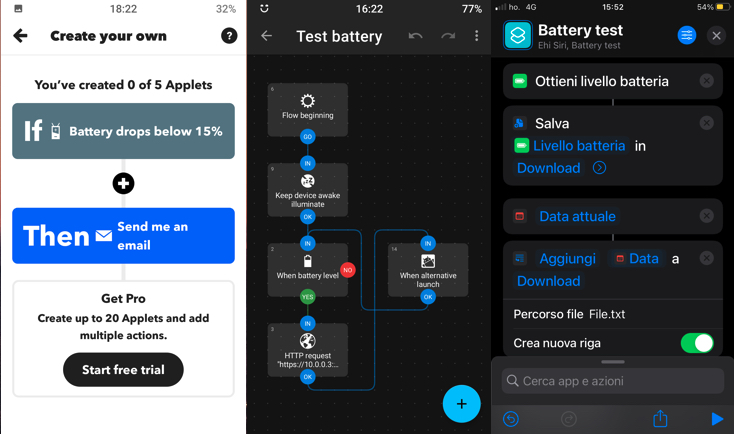
\includegraphics[width=15cm]{statoArte}
        \caption{IFTTT, Automate, Shortcuts}
        \label{fig:usecase}
    \end{figure}

    Byce offre un'alternativa già pronta all'uso senza richiedere particolari conoscienze o presentare difficili interazioni all'utente, il sistema realizzato è completamente open source\footnote[6]{Codice open source: codice disponibile pubblicamente e libero da vincoli di Copyright.} e adottabile da varie tecnologie in più scenari.
    Attualmente l'applicativo client è stato costruito e validato solamente per la piattaforma Android, però, come verrà specificato nel capitolo seguente, la tecnologia adottata consente una facile estendibilità ad iOS.\\
    Il server può essere rappresentato da qualsiasi personal computer, senza necessitare una connessione di rete Internet.\\


\chapter{Sviluppo applicativo}
    In questo capitolo verrà trattata l'implementazione delle tecnolgie scelte per realizzare l'intero sistema, quindi sia l'applicativo mobile che il server.

    Lo scambio di messaggi avviene sfruttando la tecnlogia Wi-Fi\footnote[1]{Wi-Fi: Wireless Fidelity, uno standard di rete basato sullo scambio di dati mediante onde radio e quindi assente da un canale fisico.} all'interno di una rete locale privata, con indirizzi IPv4 di classe A (10.0.0.0/24).

    \section{L'app}

        I sistemi operativi presenti sulla maggior parte di tablet e smartphone sono Android e iOS, il primo è un progetto open source fornito mediante licenza Apache\footnote[2]{Apache Software Foundation: una coprorazione Americana senza scopo di lucro che mantiene e supporta numerosi progetti open source.} e commercializzato principalmente da Google; il secondo è un software totalmente close source di proprietà dell'azienda Apple.

        In seguito a questa considerazione e alla metodologia di sviluppo adottata, si è deciso di costruire l'applicativo mediante una tecnologia ibrida, quindi realizzare un'app multipiattaforma. Per raggiungere questo scopo vi sono numerose possibilità, soprattutto basate sul linguaggio di programmazione JavaScript, infatti la soluzione scelta è l'uso del framework\footnote[3]{Framework web: software che consente l'esecuzione di applicativi web al di fuori del browser.} Cordova.


    \subsection{Funzionalità}

        Come definito nella fase di analisi, l'applicazione monitorerà lo stato della batteria ad ogni variazione, ovvero quando avviene un cambiamento del livello di carica, oppure quando il dispositivo viene alimentato o scollegato da una fonte di alimentazione esterna.

        Il device per poter inviare l'informazione rilevata deve essere autorizzato, tale conesenso avviene condividendo la password inserita dall'utente con il server, quest'ultimo deciderà quindi se autenticare il client.\\
        Di conseguenza, i dispositivi mobili inviano due tipologie di messaggi: di autenticazione oppure di informazione.

    \subsubsection{Pacchetto di autenticazione}
        I messaggi di autenticazione oltre alla password comprendono ulteriori caratteristiche necessarie a identificare i client.

        Tali informazioni sono:
        \begin{itemize}
            \setlength{\itemsep}{1pt}
            \item UUID\footnote[4]{UUID: Universal Unique Identifier è un'etichetta generata univocamente ed è indipendente da autorità di registrazione come invece può accadere con il MAC address.}: una stringa di 16 caratteri esadecimali, che identifica univocamente il dispositivo.
            \item OS Version: la versione del sistema operativo in uso (es. \textit{``Android 9''}, \textit{``iOS 15''}).
            \item Model: il modello dello smartphone o tablet in questione (es. \textit{``iPhone 13''}, \textit{``Samsung Galaxy 5''}).
            \item Name Device: il nome assegnato al client dall'utente (es. \textit{``iPhone di Alby''}, \textit{``MioAndroid''}).
        \end{itemize}

    \subsubsection{Pacchetto di informazione}
        I messaggi di informazione condividono lo stato della batteria ottenuto in seguito a uno degli eventi citati poc'anzi; è fondamentale mappare il dato in un contesto temporale, per questo ogni pacchetto comprenderà un timestamp\footnote[5]{Timestamp: una sequenza di caratteri costituita da una data e/o un orario utilizzata per identificare un'evento in una linea temporale.} generato al momento dell'invio.
        Inoltre, i pacchetti includeranno anche l'UUID per poter associare il dato al device e la password in quanto ogni messaggio deve essere autentico.



    \subsection{Apache Cordova}
        Il framework Cordova nasce nell'azienda Nitobi, acquisita da Adobe System nel 2011 la quale rinomina il progetto in \textit{``Phone Gap''}, per poi rilasciarlo in versione open source sotto licenza Apache nuovamente con il nome \textit{``Apache Cordova''}.

    La creazione del progetto è immediata tramite il comando da terminale \texttt{`\$ cordova create Byce'}.

    Il punto di forza del framework risiede nella sua semplicità, poiché lo sviluppo applicativo è costituito principalmente da 3 file:
    \begin{itemize}
        \setlength{\itemsep}{1pt}
      \item index.html, nel quale si stila l'interfaccia grafica attraverso HTML.\footnote[6]{HTML: HyperText Markup Language, standard utilizzato per creare il layout di pagine web.}
      \item index.js, file JavaScript dove si sviluppano le funzioni desiderate.
      \item config.xml, un documento XML\footnote[7]{XML: Extensible Markup Language, un linguaggio a marcatori che contiene e definisce dati arbitari in un linguaggio comprensibile sia dall'uomo che dalla macchina.} che descrive la configurazione generica dell'app, come per esempio il nome, l'icona e informazioni correlate.
    \end{itemize}


    \newpage

    All'interno del file JavaScript è obbligatorio dichiarare l'ascoltatore che chiamerà la funzione principale non appena l'applicativo viene avviato:
\begin{lstlisting}
document.addEventListener('deviceready', onDeviceReady, false);
\end{lstlisting}

    Per integrarsi facilmente con il sistema operativo sono richieste alcune librerie (chiamate plugin), quindi eseguendo da terminale il comando \texttt{`\$ cordova plugin add {{nome-plugin}}'} è possibile includere i componenti necessari, ovvero:
    \begin{itemize}
        \setlength{\itemsep}{1pt}
        \item `cordova-plugin-battery-status', il quale consente di monitorare lo stato della batteria del device.
        \item `cordova-plugin-device', che fornisce le caratteristiche utilizzate per identificare il dispositivo.
        \item `cordova-plugin-background-mode', libreria che permette l'esecuzione dell'app in background.
        \item `cordova-plugin-advanced-http', che si occupa di instaurare la comunicazione di rete tramite richieste `POST' del protocollo HTTPS.
    \end{itemize}

    \subsection{Android}

        La realizzazione dell'APK\footnote[8]{APK: Android application package è il formato che definisce il pacchetto di installazione di applicazioni scritte in Java o Kotlin per il sistema operativo Android.} richiede l'aggiunta della piattaforma Android al progetto Cordova, quindi via terminale \texttt{`\$ cordova platform add Android'}; successivamente con \texttt{`\$ cordova requirements'} si ottiene una lista dei requisiti per lo sviluppo del sistema operativo aggiunto.

        Android necessità di:
        \begin{itemize}
            \setlength{\itemsep}{1pt}
            \item `Android SDK'\footnote[9]{SDK: software development kit, pacchetto software che fornisce un'insieme di strumenti di sviluppo (es. debugger, emulatori, ecc).}, per ottenere gli strumenti di sviluppo Android.
            \item `Gradle', un tool di automazione per lo sviluppo basato sul linguaggio Groovy\footnote[10]{Groovy: un linguaggio di programmazione ad oggetti distribuito con licenza Apache.}.
            \item `Java JDK' un SDK speficifico per il linguaggio Java, che ne offre l'integrazione e fornisce la presenza di una JVM\footnote[11]{JVM: Java Virtual Machine una macchina astratta che fornisce un ambiente di esecuzione dedicato nel quale può essere eseguito un programma Java.}.
        \end{itemize}

        Una volta soddisfatti i requisiti elencati, è possibile costruire l'APK con \texttt{`\$ cordova build'}, comando che genera il pacchetto installativo per ogni piattaforma aggiunta.

            \subsubsection{Permessi di sistema}

            Per motivi di sicurezza e di privacy, i sistemi operativi obbligano i vari programmi a richiedere il permesso all'utente per poter accedere a specifici contenuti o sensori presenti nei dispositivi.
            L'unica richiesta che Byce effettua è la possibilità di mantenere l'esecuzione in background.

            Android per tale scopo fornisce un file XML ben specifico, denominato 'AndroidManifest.xml', però, al suo interno non si dichiarano solamente le user-permission bensì anche comportamenti invisibili all'utente come ad esempio l'accesso alla rete.
            Cordova si occupa in autonomia di aggiungere relative voci, ma spesso viene richiesto l'intervento del programmatore.

        \subsubsection{UUID}
            La generazione dell'UUID utilizzato per identificare i vari dispositivi può variare a seconda della versione di Android:
            \begin{itemize}
                \setlength{\itemsep}{1pt}
                \item Fino alla versione 7, l'UUID viene generato casualmente al primo avvio del dispositivo e resta invariato.
                \item Da Android 8 in poi, l'UUID è una combinazione della firma applicativa, l'utente e del dispositivo in uso; varia nel caso si cambi la chiave utilizzata per firmare l'app oppure se si ripristina il device alle impostazioni di fabbrica (factory reset).
            \end{itemize}
            Quindi è necessario firmare l'apk creata, tale azione dichiara e garantice che il software non è stato corrotto o alterato fino a quel momento, se così fosse la firma risulterebbe errata rispetto al codice presente in quanto tale validazione avviene mediante un hash crittografico.\\


        \graphicspath{ {./img/} }
        \begin{figure}[h]
            \centering
            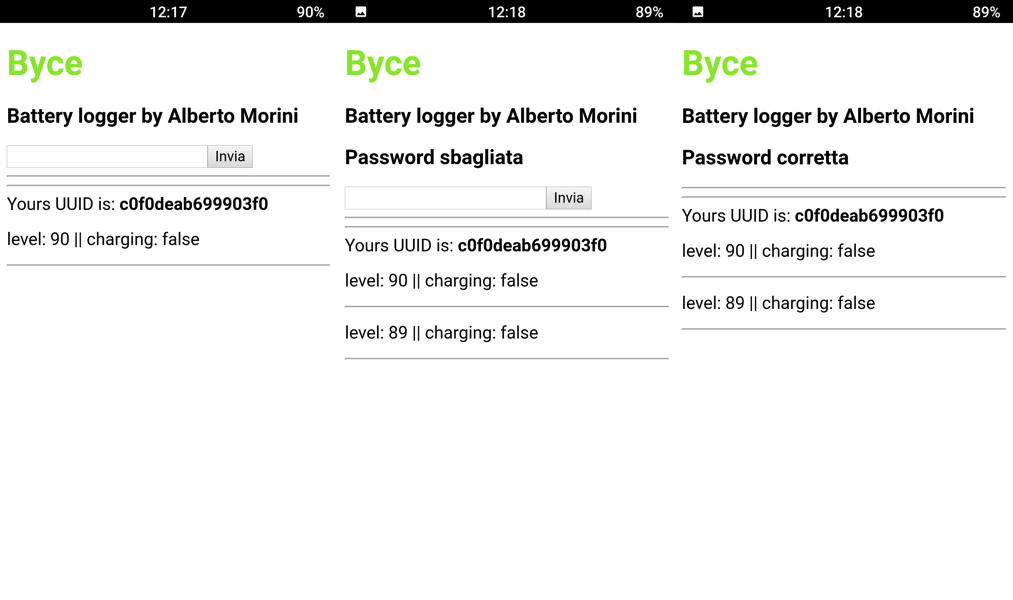
\includegraphics[width=15cm]{byceGUI}
            \caption{L'app Byce in vari scenari}
            \label{fig:usecase}
        \end{figure}

\newpage

    \section{Il server}

        Il server non è altro che un semplice personal computer, l'esecuzione del software crea due socket\footnote[12]{Socket: un'associazione costituita da un'indirizzo IP e un numero di porta che identifica un processo di rete in esecuzione su un dispositivo.} all'indirizzo IP locale, il quale viene configurato staticamente vista l'assenza di un DNS privato.

        Le porte utilizzate sono la \texttt{8124} per la registrazione dei dati rilevati e la \texttt{8127} per l'autenticazione, su quest'ultima vi sarà l'unico processo abilitato a inviare messaggi verso i client, poiché l'autorizzazione viene assegnata via medesimi pacchetti HTTPS.

        Durante la prima esecuzione, il server richiede la creazione della password di autenticazione, la quale verrà cifrata tramite la funzione di hash "MD5" e successivamente ne verrà memorizzato il risultato all'interno di un file.
        Quindi, alla ricezione di un messaggio, il server esegue l'hash della password presente nel pacchetto, per poi confrontarla con il digest\footnote[13]{Digest: l'output fornito da una funzione di hash.} esistente; se le password coincidono, il pacchetto verrà processato opportunamente, salvando i dati rilevati nel caso di un pacchetto di informazione oppure fornendo l'autenticazione e registrando il device se sconosciuto (un nuovo client).


            \subsection{NodeJS}
                NodeJS è un progetto open source multipiattaforma, il quale permette consente con l'interprete V8 di Chromium\footnote[14]{Chromium: browser gratuito e open source sviluppato e mantenuto principalmente da Google.} l'esecuzione di programmi back-end sviluppati in JavaScript.

                Node utilizza una programmazione asincrona, quindi senza attendere il termine di una operazione può procedere alla successiva, parallelizzando così la gestione delle richieste ricevute dai dispositivi e ottimizzando l'uso della memoria del computer.
                Inoltre, l'adozione del medesimo linguaggio del client a livello server offre un'ottima integrazione tra i sistemi, poiché i messaggi scambiati sono codificati con un content-type JSON, standard fortemente implementato nella tecnologia scelta.

                Sono disponibili gratuitamente svariate librerie (chiamate moduli), utilizzate per interfaccarsi con componenti del computer oppure con altri software; con la parola chiave \texttt{require(`modulo')} si includono quindi le funzioni presenti nella relativa libreria.

                I moduli richiesti al server Byce sono i seguenti:
                \begin{itemize}
                    \setlength{\itemsep}{1pt}
                    \item \texttt{var https = require(`https')}, modulo che implementa il protocollo HTTPS.
                    \item \texttt{var mysql = require(`mysql')}, per interagire con il database creato.
                    \item \texttt{var fs = require(`fs')}, per interfacciarsi con il filesystem.
                    \item \texttt{var crypto = require(`crypto')}, libreria che fornisce funzioni crittografiche tra cui MD5.
                    \item \texttt{var readline = require(`readline')}, che consente di ricevere un'input via terminale da parte utente (utilizzato nella creazione della password di autenticazione).
                \end{itemize}

                In fine, l'esecuzione del programma sviluppato avviene tramite il comando da terminale \texttt{ `\$ node server.js'}.

                \subsubsection{NPM}
                NPM è il gestore pacchetti di Node, si occupa di installare, aggiornare o rimuovere programmi e librerie in maniera consistente; Tutti i moduli citati poc'anzi sono disponibili attraverso linea di comando con \texttt{`\$ npm install {{nome-libreria}}'}.
                Inoltre, viene utilizzato anche per l'installazione del framework Cordova, utilizzato nello sviluppo client.


            \subsection{Il database}
                La base di dati utilizzata viene gesita attraverso il DBMS\footnote[15]{DBMS: Database Management System, software che consente la gestione e quindi anche la creazione di un database.} MySql di Oracle, scelta dettata principalmente dal modulo NodeJS ben documentato, nonché per sue ottime prestazioni e semplicità.

                Una volta installato e avviato il servizio, l'accesso può avvenire via terminale con \texttt{`\$ mysql -u root -p'}, quindi si inserisce la password utente di sistema.

                La creazione del database si effettua con la query \texttt{`CREATE DATABASE BYCE;'} mentre le entità necessarie sono rappresentate dalle tabelle: `DEVICES' e `DATALOG', che in quest'ordine memorizzano le caratteristiche dei client e le informazioni rilevate.

\begin{lstlisting}
CONNECT BYCE; --per utilizzare il dabase creato
CREATE TABLE DEVICES(
    UUID VARCHAR(16) PRIMARY KEY,
    NAME_DEVICE VARCHAR(128),
    MODEL VARCHAR(128),
    OS_VERSION VARCHAR(128)
);

CREATE TABLE DATALOG(
    UID VARCHAR(16) NOT NULL,
    LOG_DATE DATE NOT NULL,
    LOG_TIME TIME NOT NULL,
    BAT_LEVEL INTEGER NOT NULL,
    IN_CHARGE BOOLEAN NOT NULL,
    PRIMARY KEY (UID, LOG_DATE, LOG_TIME, BAT_LEVEL, IN_CHARGE),
    FOREIGN KEY(UID) REFERENCES DEVICES(UID)
);
\end{lstlisting}

                Come chiave primaria per i dispositivi si sfrutta l'attributo `UUID', un valore pressoché unico, la probabilità che esista una duplicazione della stringa generata non è zero, ma vicina abbastanza da essere ignorata; inoltre, la possibilità che un'utente possieda dei device che generino lo stesso UUID diminuisce nettamente la probabilità di tale casistica.

                La tabella `DATALOG' viene identificata univocamente dall'insieme di tutti gli attributi presenti, tale soluzione può essere più onerosa rispetto all'utilizzo di un'intero che incrementa in automatico, però offre una consistenza maggiore dei dati evitando inserimenti duplici (vedesi la sezione di sicurezza).
                Il livello di batteria e lo stato di alimentazione possono sembrare superflui, ma invece sono necessari poiché può accadere che lo stato di carica vari molto velocemente, ad esempio nel caso di una batteria difettosa o di un calo di corrente.

                Il server attraverso il modulo Node, esegue solamente l'operazione di inserimento nel database, in seguito se ne riporta un'esempio.
\begin{lstlisting}
//creazione della connessione
var con = mysql.createConnection({
  host: "localhost",
  user: "root",
  password: "Fixed23",
  database: "BYCE"
});

con.connect(function(err) {
      if (err) throw err;

      var sql = "INSERT INTO DATALOG(UID,LOG_DATE,LOG_TIME,BAT_LEVEL,IN_CHARGE) VALUES ('" + dataPack.UID+"','"+dataPack.LOG_DATE+"','"+dataPack.LOG_TIME+"',"+
      dataPack.BAT_LEVEL+","+dataPack.INCHARGE+");";

      //esecuzione della query
      con.query(sql, function (err, result) {
        if (!err){
            console.log("\tInfo stored into db");
        }else{
            console.log(err);
        };
      });
 });

\end{lstlisting}
            \subsection{Grafana}

                    Le informazioni raccolte vengono mostrate all'utente mediante Grafana, un'applicazione web in grado di leggere i dati da un database, analizzarli e in fine rappresentarli attraverso un'inforgrafica interattiva.\\
                    Il software open source è self-hosted\footnote[16]{Self-hosted: software eseguibili e mantenuti su server privati come un personal computer.} (come MySql) e disponibile alla porta \texttt{3000} del server; l'accesso è protetto da username e password la quale sarà obbligatorio modificare durante il primo accesso.
                    Terminata la configurazione iniziale è possibile creare una dashboard che conterrà i vari pannelli, uno per ogni informazione che si desidera trattare.

                    \graphicspath{ {./img/} }
                    \begin{figure}[h]
                        \centering
                        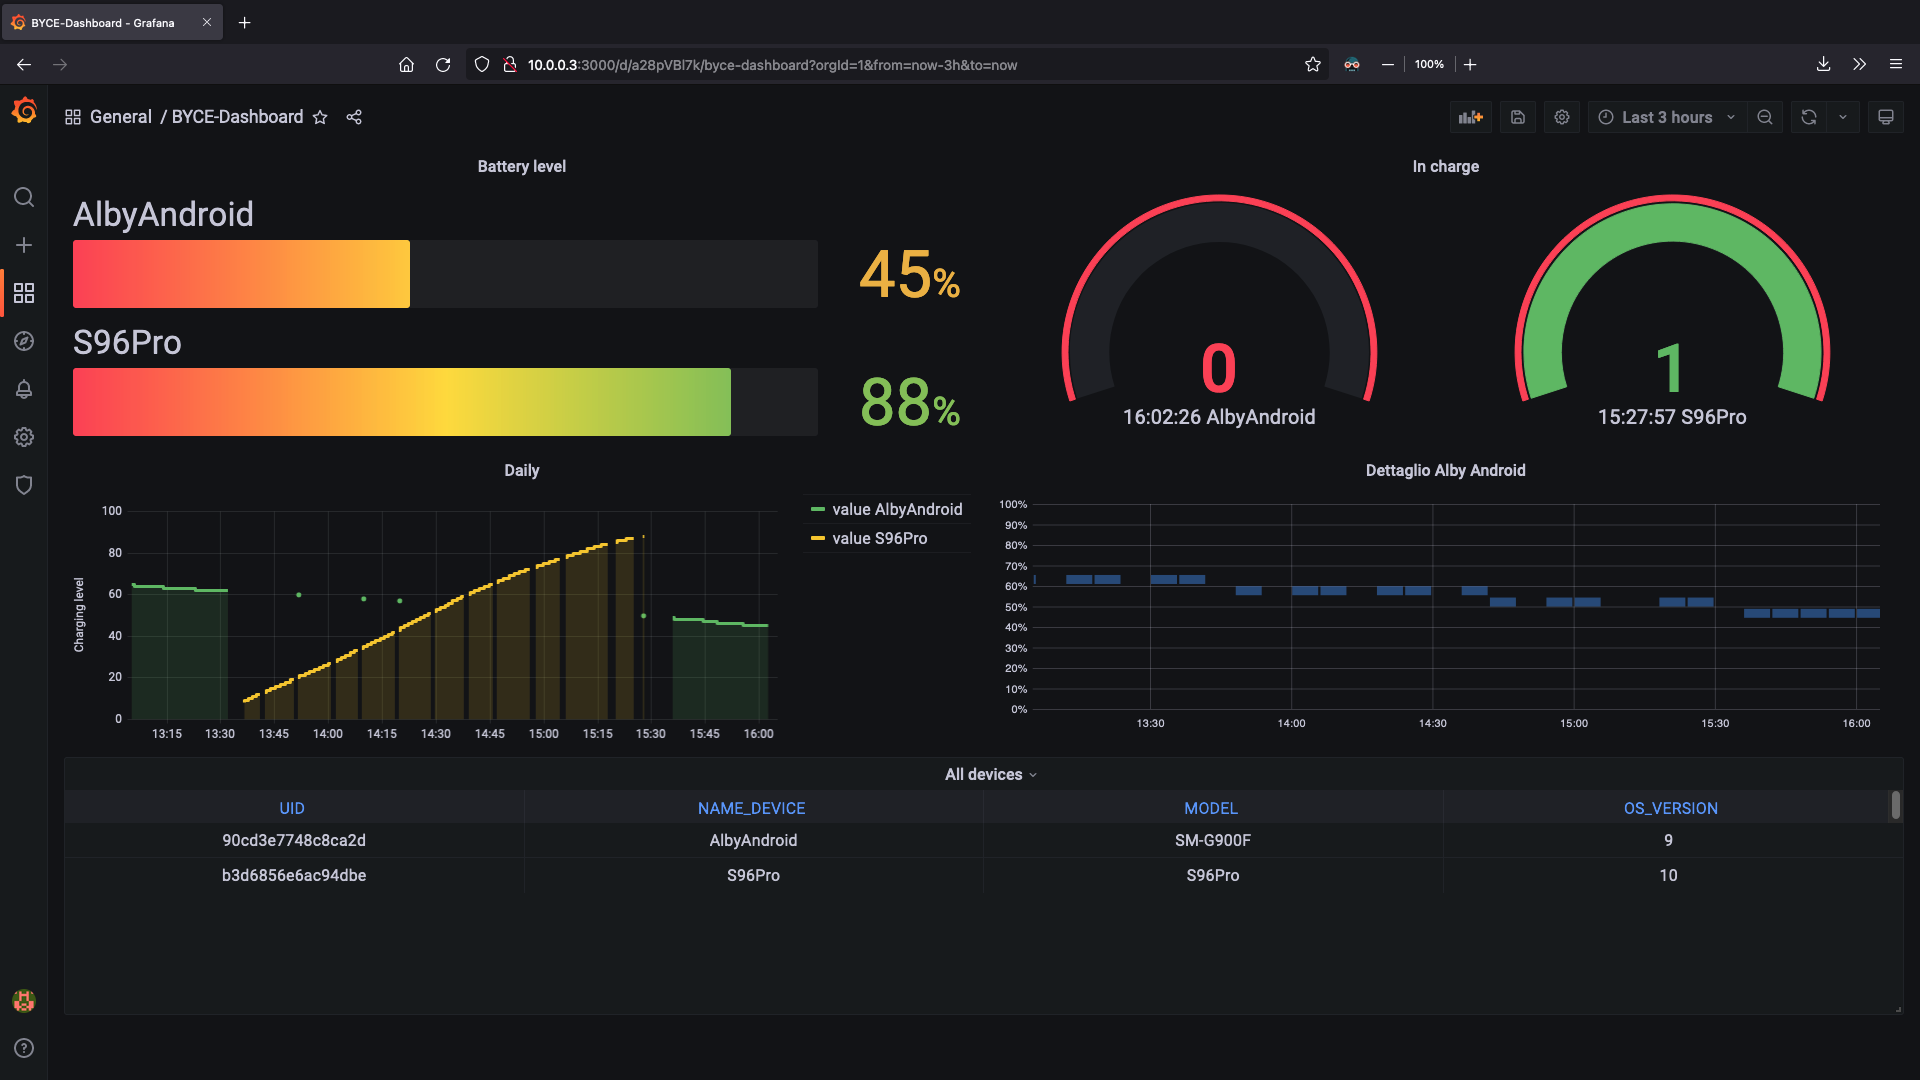
\includegraphics[width=15cm]{grafanaShot}
                        \caption{Dashboard grafana}
                        \label{fig:Infografica di Grafana }
                    \end{figure}
                    \newpage
                    La dashboard in figura mostra i dati delle ultime 3 ore dei dispositivi registrati, i quali all'orario della schermata (16:10) erano alimentati da una fonte esterna per \textit{`S96Pro'} e a batteria per \textit{`AlbyAndroid'}.


                    I pannelli sviluppati distribuiscono visivamente i dati ottenuti dalle seguenti query:
\begin{lstlisting}
SELECT BAT_LEVEL, NAME_DEVICE FROM DATALOG DL1
INNER JOIN DEVICES D ON D.UID = DL1.UID
WHERE DL1.LOG_DATE=CURRENT_DATE AND NOT EXISTS (SELECT * FROM DATALOG DL2 WHERE
    DL1.UID=DL2.UID AND
     DL1.LOG_DATE=DL2.LOG_DATE AND DL1.LOG_TIME<DL2.LOG_TIME)
GROUP BY BAT_LEVEL, NAME_DEVICE;
-- Mostra l'ultimo livello di batteria rilevato dai device monitorati nella data odierna (pannello: Battery Level).

SELECT DL1.IN_CHARGE, DL1.LOG_TIME, D.NAME_DEVICE FROM DATALOG DL1
INNER JOIN DEVICES D ON DL1.UID=D.UID
WHERE DL1.LOG_DATE=CURRENT_DATE AND
NOT EXISTS(SELECT * FROM DATALOG DL2 WHERE
DL1.LOG_TIME<DL2.LOG_TIME AND
DL1.UID=DL2.UID AND
DL1.LOG_DATE=DL2.LOG_DATE);
-- Fornisce un cruscotto dello stato di alimentazione dei device (pannello: In charge).

SELECT UNIX_TIMESTAMP(LOG_TIME) AS time_sec, BAT_LEVEL AS value, NAME_DEVICE
FROM DATALOG DL1
INNER JOIN DEVICES D1 ON D1.UID=DL1.UID
WHERE DL1.LOG_DATE=CURRENT_DATE
GROUP BY time_sec, value, NAME_DEVICE
ORDER BY time_sec, value, NAME_DEVICE;
-- Rappresenta l'andamento del livello di batteria dei device monitorati, nella data odierna (pannello: Daily).

SELECT UNIX_TIMESTAMP(LOG_TIME) AS time_sec, BAT_LEVEL AS value
FROM DATALOG DL1
INNER JOIN DEVICES D ON D.UID = DL1.UID
WHERE NAME_DEVICE='AlbyAndroid'
GROUP BY time_sec, value
ORDER BY time_sec, value
-- Genera lo storico del livello di carica del device chiamato "AlbyAndroid" (pannello: Dettaglio Alby Android).

SELECT UUID, NAME_DEVICE, MODEL, OS_VERSION FROM DEVICES;
-- Per rappresentare tutti i dispositivi registrati (pannello: All devices).

\end{lstlisting}

\section{Il pacchetto}
    I pacchetti scambiati sono codificati con un content-type `JSON', a lato client tale codifica avviene mediante l'istruzione: \texttt{`cordova.plugin.http.setDataSerializer('json');'}, mentre il server effettua \texttt{`JSON.parse(pacchetto)'} in ricezione e in invio spedisce un pacchetto con content-type `plain/text' contenente un valore booleano per restituire l'esito dell'autenticazione.

    Un esempio di un messaggio di informazione:
\begin{lstlisting}
{
  password: 'fidelio',
  UID: 'c0f0deab699903f0',
  LOG_DATE: '2022/6/2',
  LOG_TIME: '19:27:11',
  BAT_LEVEL: '6',
  INCHARGE: 'true'
}
\end{lstlisting}


\chapter{Sicurezza informatica}
In questo capitolo verranno trattate tutte le tematiche legate alla sicurazza informatica di Byce, quindi autenticazioni e potenziali minacce, all'integrità e confidenzialità del sistema.
Come citato precedentemente, il canale comunicativo tra client e server viete instaurato mediante la tecnologia Wi-Fi in una rete locale; la sicurezza di quest'ultima è un'aspetto esterno al progetto, tuttavia per escludere potenziali attaccanti è opportuno proteggere l'accesso utilizzando una password precondivisa di tipo WPA2/WPA3\footnote[1]{WPA2/WPA3: Wi-Fi protected access, protocolli sviluppati al fine di proteggere il segnale radio emesso da una rete da potenziali ascoltatori indesiderati.}.

\section{HTTPS}
    L'acquisizione dei dati da parte server rappresenta un aspetto da tutelare contro informazioni non autentiche, poiché la base di dati deve contenere solamente rilevazioni appartenenti a dispositivi riconosciuti dall'utente finale.\\
    Per prevenire questa minaccia si adotta l'autenticazione dei pacchetti tramite una password condivisa tra server e client; l'implementazione di tale meccanismo non è sufficiente nel caso di pacchetti in chiaro (HTTP), in quanto un'attaccante in ascolto sul canale sarebbe in grado di intercettare un messaggio e analizzarlo senza difficoltà. Per questo motivo si adotta il protocollo HTTPS, che implementando TLS/SSL genera delle socket sicure che cifrano i messaggi utilizzando la chiave pubblica del destinatario e quella privata per decifrare; rendendo quindi la comunicazione confidenziale esclusivamente al server e al client (end-to-end).

    Per poter istanziare un server HTTPS che accetti tale connessione, viene richiesta una chiave pubblica utilizzabile dai client e una certificazione (standard X.509) che ne garantisca l'identità.

    Tale certificazione viene fornita (spesso a pagamento) presso una Certification Autorithy (CA), la quale si impegna ad effettuare le opportune verifiche e in seguito a rilasciare l'autorizzazione. Al fine di evitare tale processo si adotta un certificato self-signed, che vede il client fidarsi della dichiarazione del server senza confrontarla con una CA.
    Questa modalità fornisce quindi una comunicazione sicura ma non autentica, per il progetto realizzato è un buon compromesso seppur questa politica lascia spazio all'attacco `man in the middle' (trattato nella sezione successiva).
    \newpage

    La generazione di una certificazione self-signed avviene da terminale:
\begin{lstlisting}
openssl genrsa -out key.pem
openssl req -new -key key.pem -out csr.pem
openssl x509 -req -days 9999 -in csr.pem -signkey key.pem -out cert.pem
\end{lstlisting}

    Al termine del processo vengono creati i file contenenti la chiave pubblica e la certificazione, i quali dovranno essere inclusi nel codice JavaScript del server
\begin{lstlisting}
var options = {
    key: fs.readFileSync('key.pem'),
    cert: fs.readFileSync('cert.pem')
}
https.createServer(options,function(req,res){ ... });
\end{lstlisting}

    Il client come menzionato in precedenza, non deve eseguire alcuna verifica del certificato fornito, poiché non verrebbe riconosciuto da alcuna Certification Autorithy.
\begin{lstlisting}
cordova.plugin.http.setServerTrustMode('nocheck', () => {
    console.log("success, no check");
}, () => {
    console.log("Error server trust mode");
});
\end{lstlisting}


\section{Attacchi e soluzioni}

    \subsection{Man in the middle}
    L'attacco conosciuto come ``man in the middle'' è possibile a causa dell'assenza di verifica del certificato presso una CA, tale minaccia vede un'attaccante dichiararsi come il destinatario (in questo caso il server), quindi il client non eseguendo controlli si fida dell'identità ricevuta. Questa vulnerabilità si risolve utilizzando un certificato X.509 attendibile ed eseguendo le opportune verifiche con la Certification Autorithy emittente, oppure istruendo il client a riconoscere il certificato generato.\\
    \textit{Tale compromesso è stato accettato unicamente per questa tesi, nel caso di un'installazione nel mercato è opportuno adottare una delle soluzioni menzionate.}

    \subsection{Attacco di Replay}
    HTTPS utilizzando un numero di sequenza previene l'attacco conosciuto come ``replay'', dove un'attaccante invia un pacchetto intercettato in precedenza. Tuttavia nel caso il server dovesse in qualche modo ricevere informazioni già presenti nella base di dati, i vincoli di univocità imposti dalle chiavi primarie non consentirebbero l'inserimento. Mentre l'attaccante non otterrebbe alcuna informazione confidenziale dal server, poiché le risposte di autenticazione come citato precedentemente, sono semplici valori booleani.

\section{Wireshark}

    La prima versione di Byce non implementava alcuna misura di sicurezza poiché le comunicazioni avvenivano via HTTP,
    tale versione è stata confrontata con quella finale in un'analisi di pacchetti mediante il software Wireshark\footnote[2]{Wireshark: software open source che consente di visionare e quindi analizzare i pacchetti ricevuti da un computer.}.

    \graphicspath{ {./img/} }
    \begin{figure}[h]
        \centering
        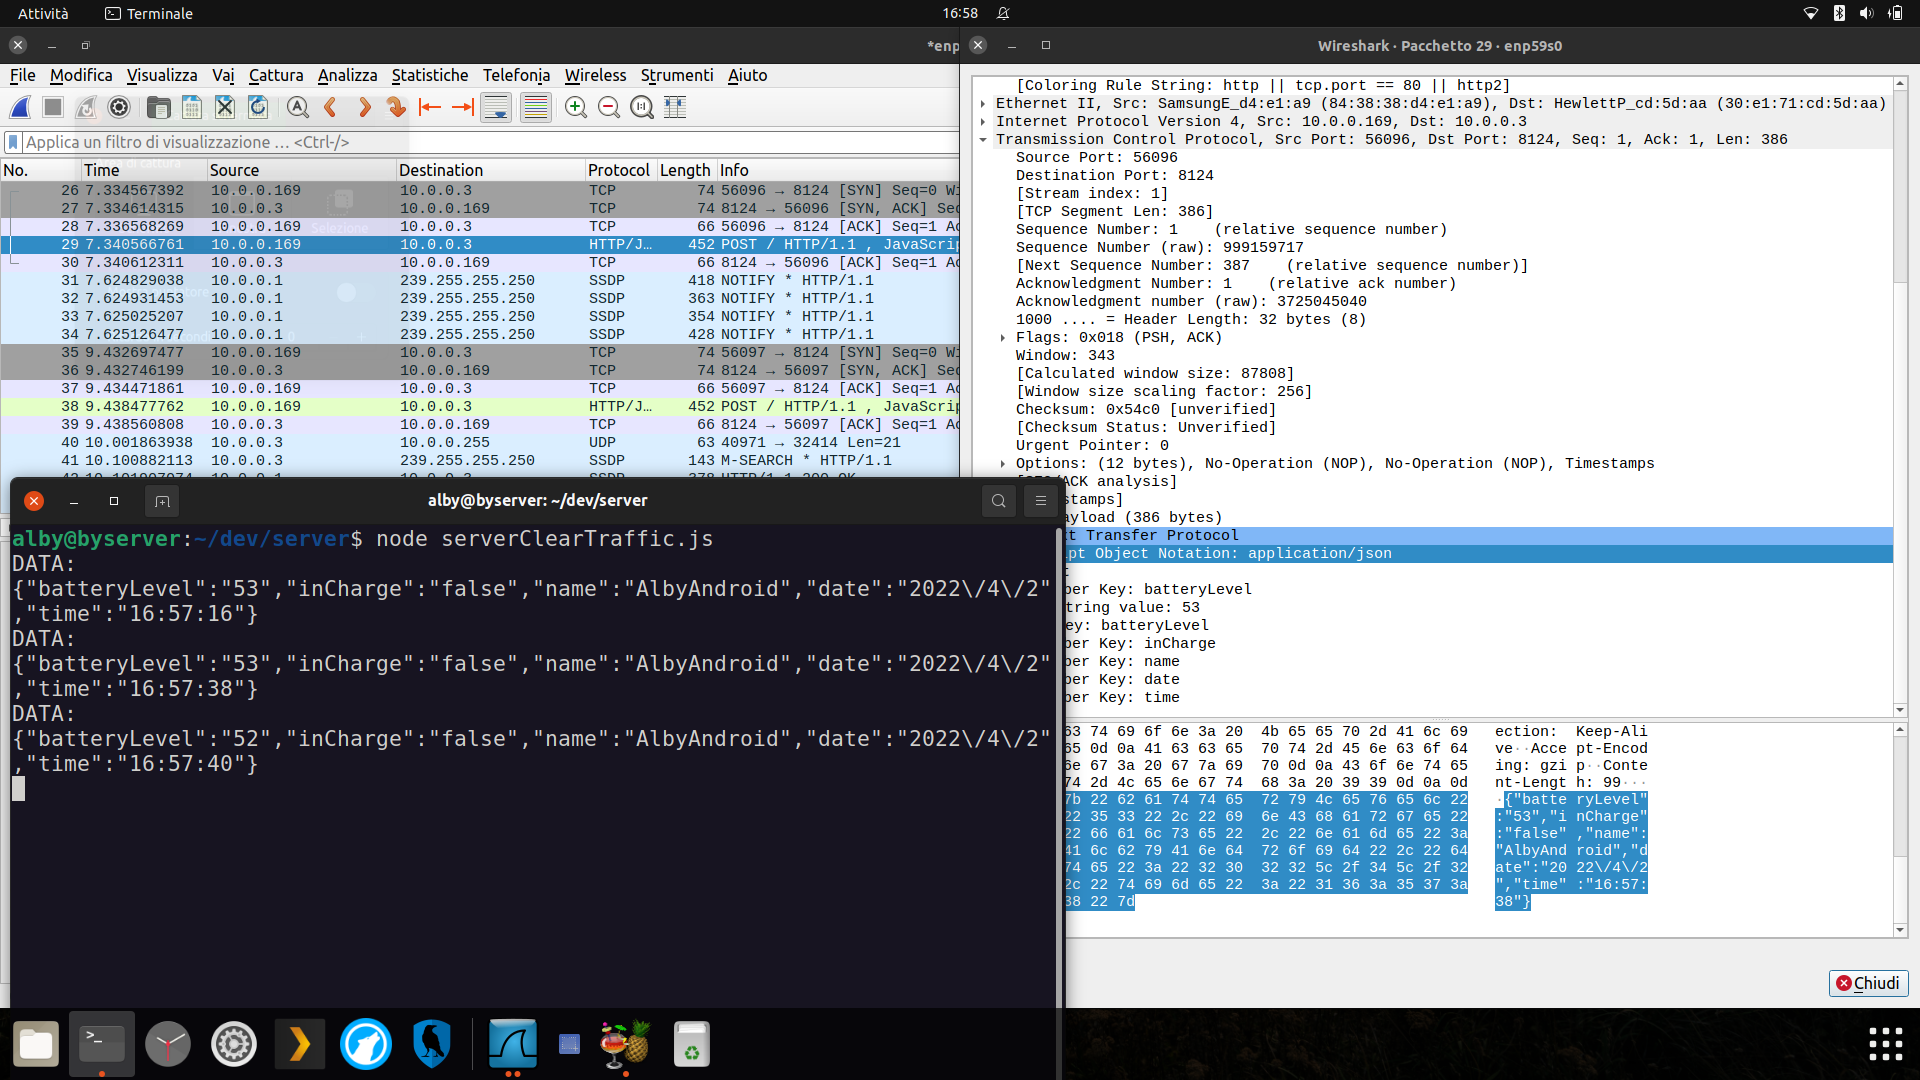
\includegraphics[width=15cm]{SniffingPacchettoInChiaro}
        \caption{Byce con HTTP}
        \label{fig:usecase}

    \end{figure}
    \graphicspath{ {./img/} }
    \begin{figure}[h]
        \centering
        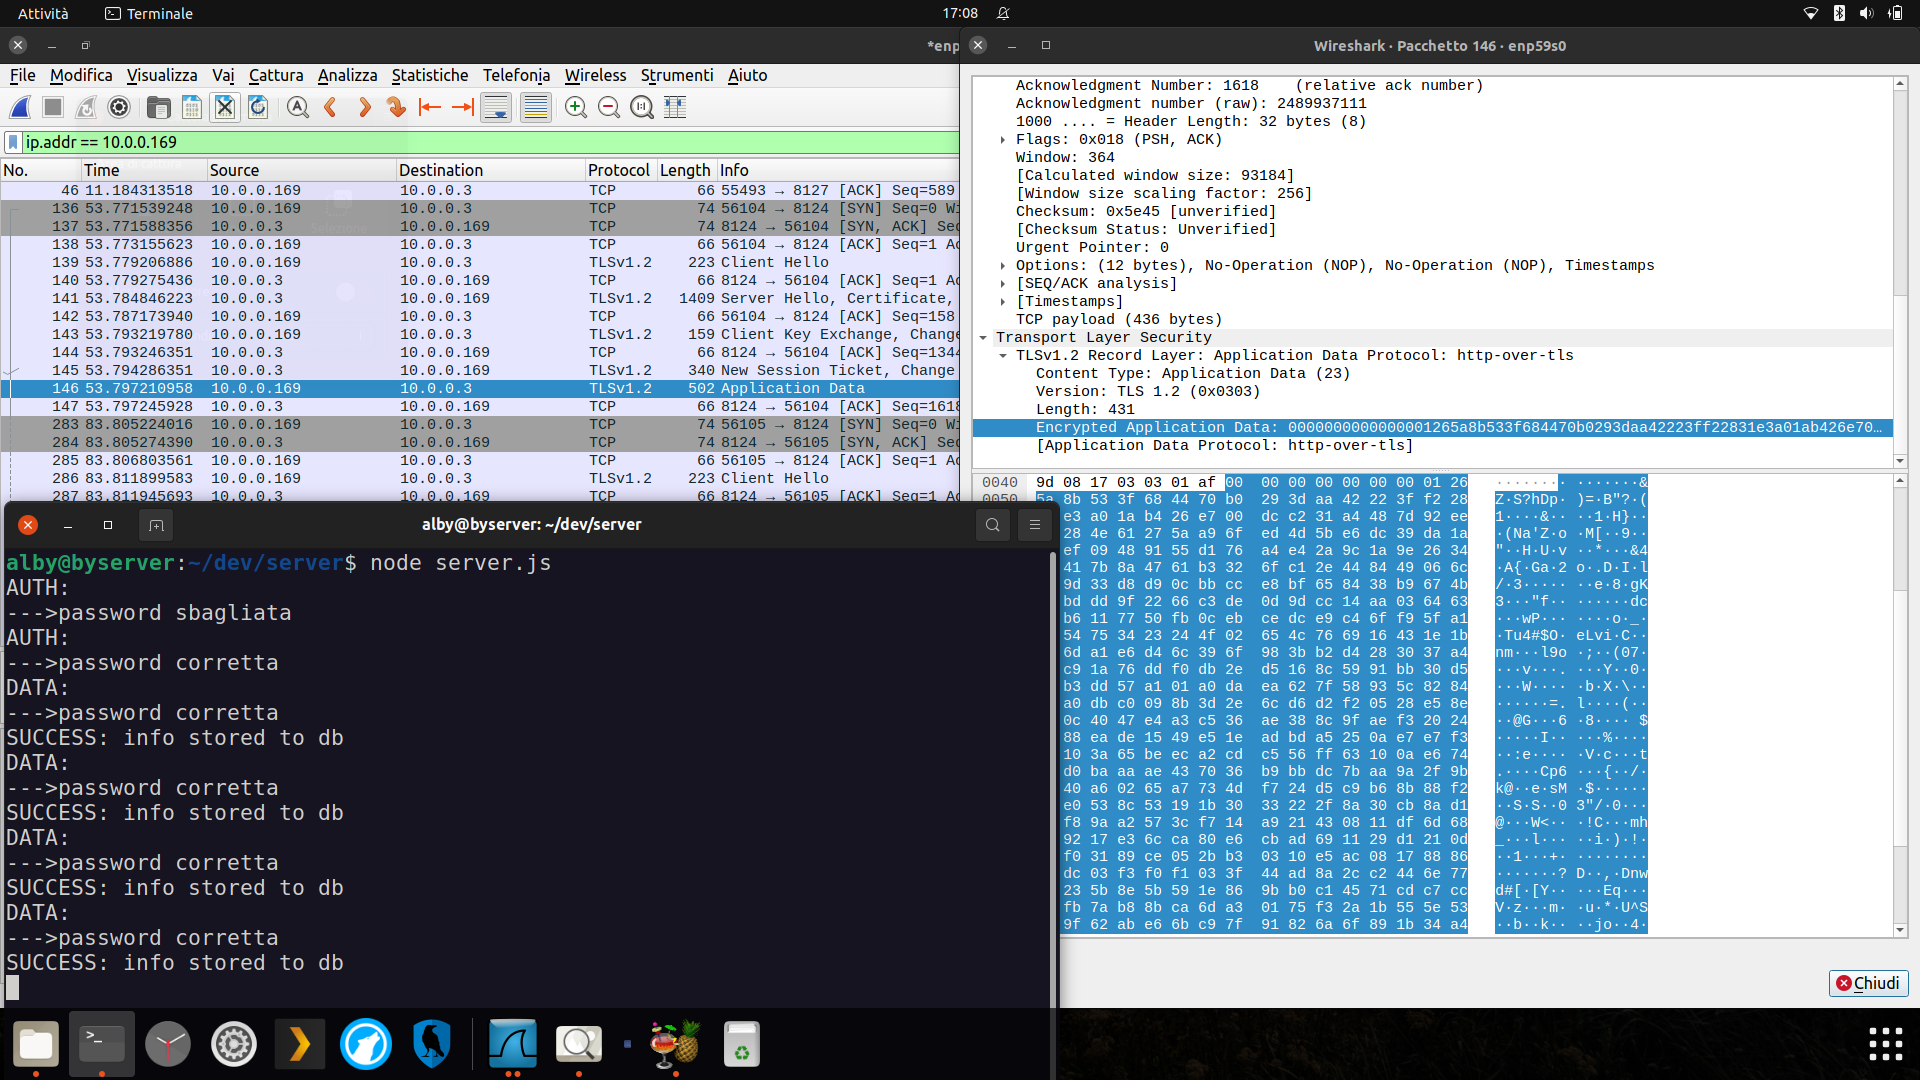
\includegraphics[width=15cm]{SniffingPacchettoCifrato}
        \caption{Byce con HTTPS}
        \label{fig:usecase}
    \end{figure}



\chapter{Conclusioni}

In conclusione, Byce vuole creare un ponte tra l'industria 4.0 e il mondo dei dispositivi mobili, con lo scopo di fornire uno strumento di analisi e monitoraggio, nonché di automatizzare compiti che possono rivelarsi noiosi per l'utente.

Come annunciato nell'introduzione, il progetto trova spazio in vari settori, in questa tesi il sistema è stato installato in un'ambiente casalingo utilizzando un semplice personal computer e alcuni smartphone.

L'intero progetto è reso disponibile sul sito: \url{https://github.com/albertomorini/Byce}

\section{Problematiche e sviluppi futuri}

\subsection{Problematiche}
Dalla versione 9 di Android, il sistema operativo interrompe totalmente l'esecuzione di un'app in background da più di circa 5 minuti, questa caratteristica purtroppo blocca l'invio dei dati.

Per aggirare questa problematica vi sono numerose strategie, la soluzione adottata consiste nell'indicare al dispositivo di non ottimizzare le risorse utilizzate da Byce, quindi nel momento in cui l'applicativo entra in background avviene la rispettiva richiesta:
\begin{lstlisting}
cordova.plugins.backgroundMode.on('activate', function() {
   cordova.plugins.backgroundMode.disableWebViewOptimizations();
});
\end{lstlisting}
Un'ulteriore alternativa implementata nelle prime versioni dell'applicativo, consiste nel portare l'app in primo piano per poi nuovamente in background ogni 5 minuti; purtroppo questa soluzione non è opportuna poiché comporta effetti non desiderati, come l'accensione del display ad ogni intervallo.


\subsection{Sviluppi futuri}

La versione attuale di Byce può essere arricchita di numerose funzionalità e soprattutto essere estesa al sistema operativo iOS.\\
Alcuni ulteriori sviluppi possono comprendere un'ampliamento dei dati rilevati, quindi non limitarsi alla monitorazione dello stato di batteria bensì anche a supervisionare risorse come l'utilizzo della CPU, quantità di memoria fisica occupata e così via.

\`E possibile integrare un sistema di analisi dei dati al fine di individuare dispositivi con batterie difettose o alimentatori mal funzionanti; inoltre registrare il tempo di ricarica elettrica dei device, realizzando quindi una business intelligence\footnote[1]{Business intelligence: insieme di strategie e tecnologie utilizzate nell'analisi dei dati per associare un costo a un componente di un sistema.} in grado di fornire all'utente una stima dei costi sostenuti.

Infine, la piattaforma Byce può essere installata in una rete WAN\footnote[2]{WAN: Wide Area Network, un'insieme di reti locali, ad esempio internet o GARR.} su un server centralizzato, quindi monitorando telefoni e tablet appartenenti a utenti diversi; offrendo sempre la possibilità di self-hosting e lasciando all'utente la scelta del server che desidera.


%% Fine dei capitoli normali, inizio dei capitoli-appendice (opzionali)
\appendix


%\part{Appendici}

%%\chapter{Titolo della prima appendice}

%% Parte conclusiva del documento; tipicamente per riassunto, bibliografia e/o indice analitico.
\backmatter




\begin{thebibliography}{9}
\bibitem{latexdps}
    Sito ufficiale di Apache Cordova: \url{https://cordova.apache.org/}
\bibitem{texbook}
    Documentazione Shortcuts di Apple: \url{https://support.apple.com/guide/shortcuts/welcome/ios}\\
    \textit{Il download è unicamente disponibile tramite lo store ufficiale:} \url{https://apps.apple.com/us/app/shortcuts/id915249334}.
\bibitem{latexdps}
    Pagina principale di IFTTT: \url{https://ifttt.com/explore}
\bibitem{latexdps}
    Sito ufficiale con documentazione per Automate di LlamaLab: \url{https://llamalab.com/automate/}
\bibitem{latexdps}
    NodeJS e NPM: \url{https://nodejs.org/en/}
\bibitem{latexdps}
    Sito web di Grafana Visualization: \url{https://grafana.com/grafana/}
\bibitem{latexdps}
    Sito ufficiale di MySql: \url{https://www.mysql.com/}
\bibitem{latexdps}
    Java Development Kit \url{https://www.oracle.com/java/technologies/}
\bibitem{latexdps}
    Sito al tool Gradle \url{https://gradle.org/}
\bibitem{latexdps}
    Pagina officiale di Android Studio: \url{https://developer.android.com/studio/}
\bibitem{latexdps}
    Documentazione Android per firmare l'apk realizzata: \url{https://developer.android.com/studio/command-line/apksigner#usage-sign}
\bibitem{latexdps}
    Informazioni sulla generazione dell'UUID da Android 8 in poi (indicato con `ANDROID\_ID'): \url{https://developer.android.com/about/versions/oreo/android-8.0-changes#privacy-all}

\end{thebibliography}


%% Per l'indice analitico, usare il pacchetto makeidx (o analogo).

\end{document}

--- Istruzioni per l'aggiunta di nuove lingue ---
Per ogni nuova lingua utilizzata aggiungere nel preambolo il seguente spezzone:
    \addto\captionsitalian{%
        \def\abstractname{Sommario}%
        \def\acknowledgementsname{Ringraziamenti}%
        \def\authorcontactsname{Contatti dell'autore}%
        \def\candidatename{Candidato}%
        \def\chairname{Direttore}%
        \def\conclusionsname{Conclusioni}%
        \def\cosupervisorname{Co-relatore}%
        \def\cosupervisorsname{Co-relatori}%
        \def\cyclename{Ciclo}%
        \def\datename{Anno accademico}%
        \def\indexname{Indice analitico}%
        \def\institutecontactsname{Contatti dell'Istituto}%
        \def\introductionname{Introduzione}%
        \def\prefacename{Prefazione}%
        \def\reviewername{Controrelatore}%
        \def\reviewersname{Controrelatori}%
        %% Anno accademico
        \def\shortdatename{A.A.}%
        \def\summaryname{Riassunto}%
        \def\supervisorname{Relatore}%
        \def\supervisorsname{Relatori}%
        \def\thesisname{Tesi di \expandafter\ifcase\csname thud@target\endcsname Laurea\or Laurea Magistrale\or Dottorato\fi}%
        \def\tutorname{Tutor aziendale%
        \def\tutorsname{Tutor aziendali}%
    }
sostituendo a "italian" (nella 1a riga) il nome della lingua e traducendo le varie voci.
